\chapter{Spectral Method and Spectral Pollution}
\section{Spectral Method}
Spectral method is one of the best tools to solve PDE and ODE problems. \cite{trefethen_spectral_2000} The central idea of spectral method is by discretizing the equation, we can transform that to a linear system or an eigenvalue problem.

Here we reformulate the polynomial eigenvalue problem, Eq.(\ref{eq:polynomial-eigenvalue-problem}) as the following, 
\begin{equation} \label{eq:eigenvalue-problem}
	\mqty[ 0 & 1\\ \hat{M} & \hat{N} ]\mqty[ \tilde{v}\\ \omega \tilde{v}] = \omega\mqty[ \tilde{v}\\ \omega \tilde{v}]
\end{equation}
where the operators $\hat{M}$ and $\hat{N}$ are defined as
\begin{align*}
	\hat{M} &= -\left[(1-v_0^2)\pdv[2]{}{z} 
	-\left(3v_0 + \frac{1}{v_0}\right)\pdv{v_0}{z}\pdv{}{z} 
	- \left(1-\frac{1}{v_0^2}\right)\left(\pdv{v_0}{z}\right)^2 
	- \left(v_0+\frac{1}{v_0}\right)\pdv[2]{v_0}{z}\right] \\
	\hat{N} &= -2i\left(v_0\pdv{}{z} +\pdv{v_0}{z} \right) 
\end{align*}
This becomes an ordinary algebraic eigenvalue problem if we discretize the operators and the function $\tilde{v}$. In this thesis, finite-difference, finite-element and spectral-element discretizations are used.

\section{Spectral Pollution and Spurious Modes}
In this section, we will discuss an important phenomenon we observe throughout the numerical experiments. It is the phenomenon called spectral pollution. Then we will provide a method to filter these spurious modes.

Spectral pollution refers to the phenomenon which some eigenvalues are not converging to the correct value when the mesh density is increased. When solving eigenvalue problems using spectral methods with finite difference or finite element approximations, spectral pollution might occur. \cite{llobet_spectral_1990}

\subsection{Illustration: Constant velocity case}
We will illustrate the spectral pollution by solving Eq.(\ref{eq:polynomial-eigenvalue-problem}) with constant velocity profile, $v_0=\text{const}$, using spectral method with finite-difference method.

Let $v_0\neq 1$ be a constant, then Eq.(\ref{eq:polynomial-eigenvalue-problem}) becomes 
\begin{equation} \label{eq:constant-v-problem-dirichlet}
  \omega^2\tilde{v} + 2i\omega v_0\pdv{\tilde{v}}{z} + (1-v_0^2)\pdv[2]{\tilde{v}}{z} = 0
\end{equation}

The dispersion relation can be obtained by substituting $\tilde{v} \sim \exp(-i\omega t + kx)$ into Eq.(\ref{eq:constant-v-problem-dirichlet}),
\begin{equation} \label{dispersion-relation}
	\omega = k(v_0 \pm 1) 
\end{equation}
where $k$ is the wave number. We see that all modes should be stable for $\omega\in\mathbb{R}$.

\begin{figure}[htbp]	
  \centering
	\begin{subfigure}[b]{0.4\linewidth}
		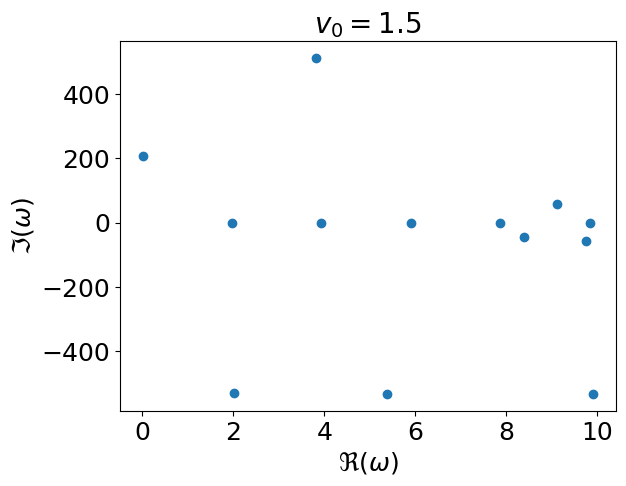
\includegraphics[width=\linewidth]{figures/eigvals-bad} 
		\caption{Unfiltered eigenvalues.}
	\end{subfigure}%
	\begin{subfigure}[b]{0.6\linewidth}
		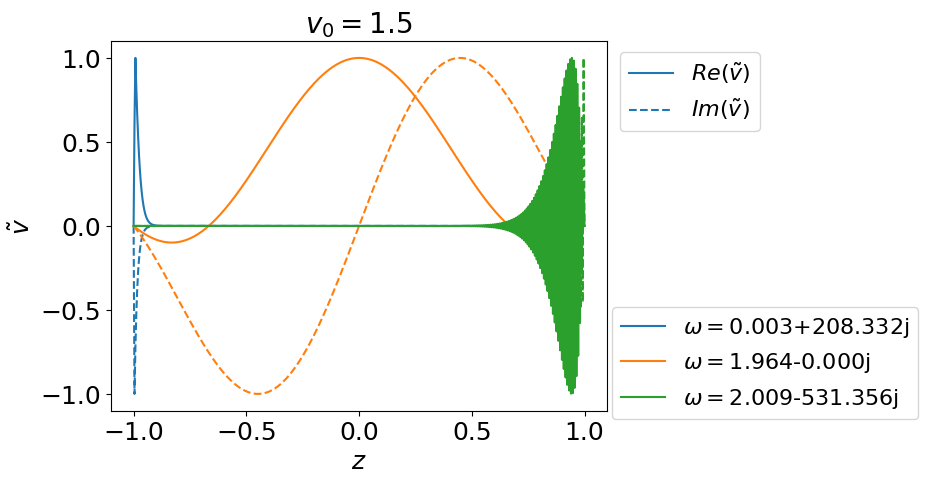
\includegraphics[width=\linewidth]{figures/eigvecs-bad} 
		\caption{First few unfiltered eigenfunctions.}
	\end{subfigure}
  \caption{Spurious modes occurs when solving Eq.(\ref{eq:constant-v-problem-dirichlet}). Finite difference discretization was used. A considerably high resolution mesh with 501 points was used. In fact, spurious modes occurs regardless of the resolution.}
	\label{fig:results-bad}
\end{figure}

A good way to filter the spurious modes is by doing a convergence test, see Fig.(\ref{fig:converging-test}). Since the eigenvalues, Eq.(\ref{dispersion-relation-G}), are changing with mesh resolution. We can simply solve the problem using spectral method under different mesh resolution. Then filter out the eigenmodes that are not converging.

\begin{figure}[htbp]
  \begin{center}
    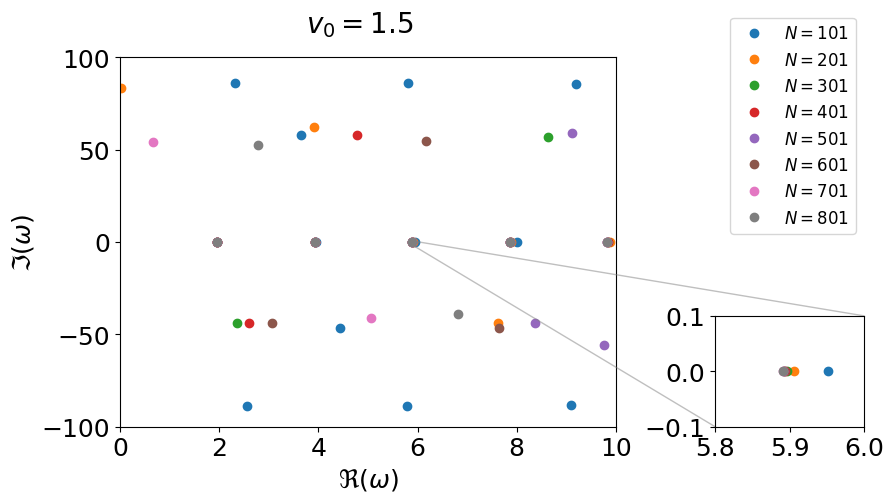
\includegraphics[width=0.7\textwidth]{figures/convergence-test.png}
  \end{center}
  \caption{Converging test works since spurious eigenvalues change under different resolution. We can see that only the eigenvalues on the real axis are not changing dramatically when resolution increases.}
  \label{fig:converging-test}
\end{figure}


\begin{figure}[htbp]
	\centering
	\begin{subfigure}[b]{0.4\linewidth}
		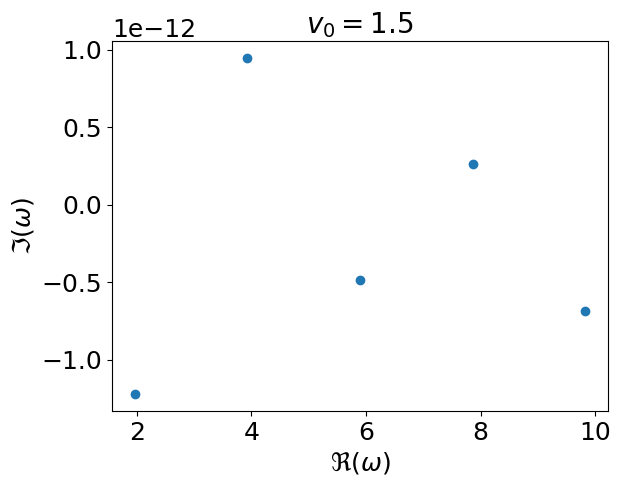
\includegraphics[width=\linewidth]{figures/eigvals-good} 
		\caption{Filtered eigenvalues.}
	\end{subfigure}%
	\begin{subfigure}[b]{0.6\linewidth}
		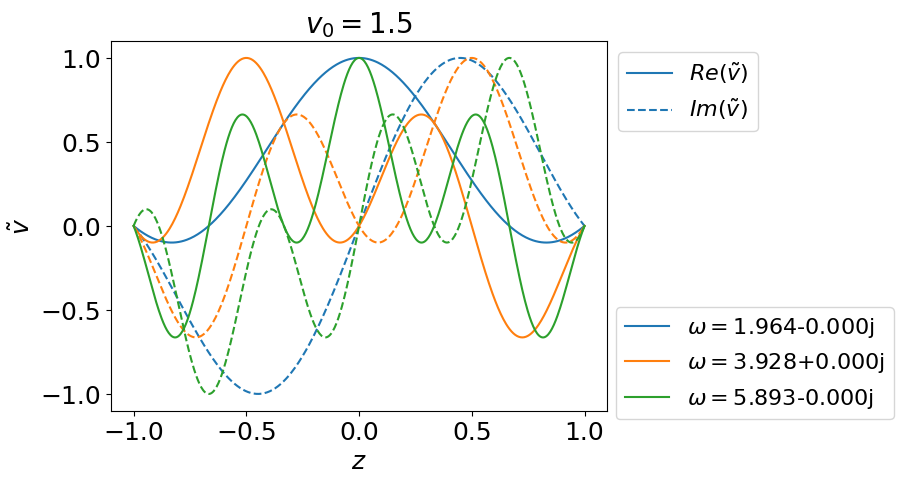
\includegraphics[width=\linewidth]{figures/eigvecs-good} 
		\caption{First few filtered eigenfunctions.}
	\end{subfigure}
	\caption{Filtered spurious modes by converging test.}
	\label{fig:results-good}
\end{figure}

